\documentclass[twocolumn]{IEEEtran}
\usepackage{graphicx}
\usepackage[utf8x]{inputenc}
\usepackage{times}
\usepackage{amssymb,amsfonts}
\usepackage[tbtags]{amsmath}
\usepackage{cite}
\usepackage{pict2e}
\usepackage{float}
\usepackage{lscape}
\usepackage[all]{xy}
\usepackage{graphics,graphicx,color,colortbl}
\usepackage{times}
\usepackage{subfigure}
\usepackage{wrapfig}
\usepackage{multicol}
\usepackage{cite}
\usepackage{url}
\usepackage[tbtags]{amsmath}
\usepackage{amsmath,amssymb,amsfonts,amsbsy}
\usepackage{listings}
\usepackage{bm}
\usepackage[centerlast, small]{caption}
\usepackage[colorlinks=true, citecolor=blue, linkcolor=blue, urlcolor=blue, breaklinks=true]{hyperref}
\hyphenation{ele-men-tos he-rra-mi-en-ta cons-tru-yen trans-fe-ren-ci-a pro-pu-es-tas si-mu-lar vi-sua-li-za-cion}

\begin{document}

\title{Brazo robótico multipropósito}
\author{José Alejandro Logreira Ávila Código: $261722$\\
	David Ricardo Martínez Hernández Código: $261931$\\
	Edwin Fernando Pineda Vargas Código: $262100$}
\maketitle
\markboth{Universidad Nacional de Colombia}{}
\floatname{algorithm}{Algoritmo}
\begin{keywords}
 Brazo, Control, FPGA, Servo-Motor, Periférico, Procesador LM32, PWM.
\end{keywords}
\begin{abstract}
 Se implementa un brazo robótico controlado por un periférico, el cual se integra una tarjeta de desarrollo \textit{``FPGA''} con su correspondiente programación para efectuar múltiples tareas, tales como mover objetos con un peso no mayor a $200 g$.
\end{abstract}

\section{Introducción}
\noindent
El uso de la tecnología para incentivar el desarrollo de la educación y diversión de las nuevas generaciones es reciente.\\\\
Desde los años $70$´s, estos desarrollos se ha iniciado utilizando diversos componentes como la programación de computadoras, creación de modelos a escala, e inclusive simulando grandes retos de ingeniería o medicina, tales como construcciones, operaciones, simulación de vuelos, estrategias militares, dando así la oportunidad de una interacción directa entre los niños y la realidad de su entorno. Incentivando la creatividad y brindandoles la oportunidad a temprana edad, de encaminarse hacia una de las múltiples disciplinas que tenemos en la actualidad, mediante la toma de desiciones de manera semicontrolada, de tal forma, que se recrean ambientes reales o casi reales, en los cuales no se exponen a los niños. Logrando que a futuro, podamos contar con una nueva generación que solucione de manera más eficaz problemas de alta ingeniería o sociales, basándose en sus experiencias tempranas mediante el juego, para así corregir sus errores.\\
Un gran número de expertos siguen la teoría de que los niños aprenden por medio de la creación de su propio conocimiento, asimilando los cambios que aparecen en su entorno y descubriendo continuamente cosas nuevas. Sobre esta base parece adecuado facilitar el uso de las nuevas tecnologías, que ayudarían a los niños a ir creando su propio saber al estimular o ayudar la capacidad de aprender.

\section{Estructura del sistema}
\noindent
El sistema se compone de tres partes: los actuadores que son los elementos encargados de realizar los movimientos del brazo, las entradas del usuario que son los pulsadores que indican la cantidad de movimiento de cada motor, y el sistema que controla e integra ambas partes.\\
Los actuadores son servomotores seleccionados de distintos tamaños y capaces de realizar distintos torques, según sea la articulación que maniobra. Los servomotores sólo poseen 3 terminales: alimentación, tierra y señal de control. La señal de control es la que controla la posición de los servomotores, que tienen un rango de movimiento de $180°$. Esta debe ser una señal digital modulada en PWM, cuyo ancho de pulso determina la posición del motor. El rango del ancho de pulso es entre $0.5ms$ y $2.5ms$, mientras que el periodo de la señal PWM es de $20ms$.\\
Los pulsadores que permiten el ingreso de órdenes por el usuario son un arreglo de botones ordenados de a pares, donde cada par puede controlar el movimiento de uno de los motores. La información que se recoge de cada uno de los pulsadores no es sólo la presión del mismo, sino la duración de la presión, que determina también la velocidad de giro del servomotor.\\
La unidad que controla e integra los actuadores y los servomotores es la integrada por el procesador, la memoria de programa y los periféricos de comunicación diseñados. El programa diseñado se encarga de recibir la información de la duración de pulsación de cada botón del control, y traducirla en el ancho de pulso pertinente para que el motor que se desea mover, lo haga de manera adecuada, es decir, regula la velocidad del motor. Este programa es guardado en la memoria de programa y es el procesador quien se encarga de realizar todas estas tareas. Finalmente los periféricos creados realizan la función de acondicionar la señal digital recibida (en el caso de los pulsadores) o enviada (en el caso de los servomotores), a partir de la información que les llega de los pulsadores o del procesador.

\subsection{Hardware}
\noindent
Como se mencionó anteriormente, en HW se implementaron 2 módulos genéricos para el manejo de los pulsadores y los motores.

\subsubsection{Control General con pulsadores}
\noindent
Los pulsadores comunes presentan un comportamiento de rebote cuando son oprimidos o liberados de la presión, por tanto, para evitar la lectura de múltiples presiones, se implementa un circuito antirrebote basado en el muestreo continuo de la señal del pulsador una vez se ha detectado el primer flanco de presión. Tras generar una señal filtrada (sin rebotes) del pulsador, esta es muestreada a la frecuencia de la tarjeta ($50MHz$), y con el uso de contadores se genera un vector de 32 bits que contiene el número de conteos de la presión del pulsador, es decir, contiene información de cuanto tiempo se ha presionado el botón.\\
Para este periférico se utilizó una PCB, $10$ pulsadores normalmente abiertos, $10$ resistencias de $2.2K \Omega$, $2$ conectores lineales utilizados como salidas. El impreso que se utilizo fue el mostrado en la Figura \ref{fig1}.\\
\begin{figure}[]
	\centering
		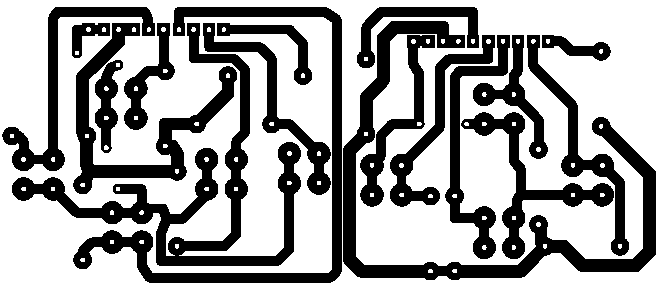
\includegraphics[scale=0.7]{Control_1_3.PDF}
	\caption{Circuito Impreso del Control General al $70\%$.}
	\label{fig1}
\end{figure}
\noindent
Este control es quien da la orden de movimiento a cada motor para poder llegar al lugar en el que se encuentra el objeto deseado.


\subsubsection{Procesador e interfaz con elementos I/O}
\noindent
Para la comunicación tanto de los pulsadores como de los motores con el procesador, se tomó como base el módulo GPIO. Este presenta un esquema de direccionamiento claro y sencillo, que se modificó para incluir los elementos de entrada y salida necesarios, añadiendo nuevos campos de dirección que dirigieran los datos tanto desde los pulsadores al procesador como de este último hacia los motores.

\subsubsection{Manejo de Servomotores}
\noindent
Los servomotores usan la señal PWM como control de posición. Esta señal tiene características que son genéricas para todos lo servomotores de naturaleza análoga, tales como su frecuencia y el rango de variación del ciclo útil. Estas características las implementa un módulo que recibe el número de cuentas de reloj (reloj de 50MHz) que equivale al ancho de pulso que se debe generar. Adicionalmente limita el rango del ciclo útil de la señal PWM, adaptándola al rango permitido.\\
Se utilizaron $3$ motores para mover la parte inicial del brazo (Hombro). De los cuales uno gira es sentido azimutal respecto al plano horizontal, los otros dos son los encargados de de girar en sentido radial. Otro motor representa el codo del brazo. Final mente en la parte superior tiene 2 motores, el primero es el encargado de dar un movimiento circular y el último de ellos abre y cierra la pinza de agarre.\\
En total se utilizaron $6$ motores en total para dar $5$ grados de libertad.
%Estructura del sistema, recursos trabajados, que se utilizo de la tarjeta de desarrollo, justificado, sacar hardware: Perifericos, memoria, procesador. Software, rutinas y subrutinas del sistema.

\section{Dificultades y Soluciones}

\subsection{Dificultades}
\begin{itemize}
 \item La estructura física y mecánica del brazo, fue muy complicada porque nunca en todo lo que se había estudiado en la carrera nos habían enseñado a construir una estructura de estas características.
  \item Durante el desarrollo del proyecto, la definición de las tareas que realizaría cada módulo del sistema no eran claras pues no se tenía claridad en el proceso de comunicación entre el programa a realizar y los distintos periféricos usados.
 \item En el marco de la comunicación entre Software y Hardware, es conveniente el conocimiento en  temas de direccionamiento de memoria a componentes externos, mapeo de memoria según tipos de datos y demás temas relacionados con la comunicación entre el procesador y sus periféricos, que no son cubiertos en el curso teórico de Electrónica Digital II. Esto representó en el proceso de selección de proyecto y su posterior inicio y desarrollo, una visión limitada de las capacidades de las que se dispone para usar el procesador con múltiples aplicaciones. 
 \item La utilización e implementación de materiales al momento de diseñar el prototipo se dificultó debido a la poca oferta de piezas mecánicas de precisión, presentes en el mercado. Además de la lejanía para obtenerlas.
 \item Las herramientas disponibles para el desarrollo de hardware son muy limitadas en nuestro país. Debido a que no se cuenta con tecnología necesaria para poder fabricar piezas de precisión. Esto genera desajustes e incomodidades al momento de ensamblarlo.
 \item Los costos para desarrollo de hardware en nuestro país son muy elevados debido a que la industria nacional no esta diseñada ni orientada a ello. Esto representa una demora significativa al momento de ensamblar un prototipo, ya que es necesario esperar la importación de algunas piezas del artículo a desarrollar.
\end{itemize}

\subsection{Soluciones}
\begin{itemize}
 \item Lo primero que todo es que es necesario una materia en el plan de estudios alguna materia que nos permita entender y diseñar este tipo de artefactos, ademas no se tenia gran conocimiento de los diferentes materiales que se pueden utilizar, tampoco sus características y ventajas más importantes.
 \item Mediante la utilización de las precarias herramientas de software con que disponemos, se pueden diseñar modelados en `$3D$, los cuales ademas de ofrecer una perspectiva del producto a desarrollar aminoran los costos, ya que de manera virtual se logra una recreación del producto.
 \item El trabajo en grupo es una de las principales herramientas que ayuda a fortalecer el desarrollo de una idea. En este proyecto en particular se utilizó en cada una de las fases que lo componen. Generando soluciones y toma de decisiones que ayudaron a concretarlo 
\end{itemize}


%Principales dificultades del proyecto, ideas para solucionar problemas, y criterios para solucionarlos

\section{Análisis Económico}
\noindent
\subsection{Costos de Ingeniería no recurrente}
\noindent
A continuación se relacionan los costos de ingeniera no recurrente correspondientes a la fase de desarrollo del producto antes de su implementación al mercado (TABLA \ref{tab1}).
\begin{table}[H]
	\centering
\begin{tabular}{|c|c|c|c|}\hline
 \textbf{Cantidad en Horas} & \textbf{Recurso} & \textbf{Valor Hora} & \textbf{Total} \\ \hline
 $50$ & Investigación & $30.000$ & $1'500.000$ \\ \hline
 $100$ & Diseño & $30.000$ & $3'000.000$ \\ \hline
 $100$ & Programación & $30.000$ & $3'000.000$ \\ \hline
 $150$ & Ensamble & $30.000$ & $4'500.000$ \\ \hline
 $50$ & Corrección a fallas & $30.000$ & $1'500.000$ \\ \hline
    \end{tabular}
	\caption{Costos no recurrentes.}
	\label{tab1}
\end{table}
\noindent
En total se invirtieron $450$ horas entre los tres integrantes del grupo, las cuales tienen un valor de $13'500.000$.

\subsubsection{Costos del prototipo}
\noindent
A continuación se relacionan los costos pertenecientes a la implementación del prototipo (TABLA \ref{tab2})
\begin{table}[H]
	\centering
\begin{tabular}{|c|c|r|r|}\hline
 \textbf{Cantidad} & \textbf{Recurso} & \textbf{Valor Unitario} & \textbf{Total} \\ \hline
 3 & Motores de $2.3 Kg/cm$ & $23.000$ & $69.000$ \\ \hline
 2 & Motores de $2.5 Kg/cm$ & $20.000$ & $40.000$ \\ \hline
 2 & Motores de $1.8 Kg/cm$ & $18.000$ & $36.000$ \\ \hline
 1 & Motor de $2.5 Kg/cm$ & $25.000$ & $25.000$ \\ \hline
 3 & Acrílico de $15cm*120cm$ & $6.000$ & $18.000$ \\ \hline
 1 & Base acrílico $15.2 cm$ & $10.000$ & $10.000$ \\ \hline
 1 & Pegante de acrílico & $7.000$ & $7.000$ \\ \hline
 1 & Rodamiento & $4.000$ & $4.000$ \\ \hline
 1 & Eje con base & $15.000$ & $15.000$ \\ \hline
 24 & Tornillos Golosos & $25$ & $600$ \\ \hline %Agregar los tornillos
 20 & Pulsadores $N/A$ & $150$ & $3.000$ \\ \hline
 16 & Resistencias a $1/2W$ & $50$ & $800$ \\ \hline
 1 & PCB de $20cm*20cm$ & $3.000$ & $3.000$ \\ \hline
 2 & Condensadores & $200$ & $400$ \\ \hline
 1 & Transformador de $120V$ a $9V$ & $15.000$ & $15.000$ \\ \hline
 1 & Diodo & $200$ & $200$ \\ \hline
 1 & Tarro de Ácido Férrico & $1.500$ & $1.500$ \\ \hline
 1 & Clavija hembra & $1.000$ & $1.000$ \\ \hline
 1 & Clavija & $1.000$ & $1.000$ \\ \hline
 1 & Un metro de cable Duplex & $3.000$ & $3.000$ \\ \hline
 2 & Ribbun & $2.500$ & $5.000$ \\ \hline
 3 & Conectores Ribbun & $1.200$ & $3.600$ \\ \hline
 30 & Conectores lineales & $100$ & $3.000$ \\ \hline
 4 & Pliegos de lija $80$ & $1.000$ & $4.000$ \\ \hline
 3 & Broca calibre $1/32''$ & $1500$ & $4.500$ \\ \hline
 1 & Broca calibre $1/64''$ & $2.000$ & $2.000$ \\ \hline
 1 & Broca $N°6$ & $2.000$ & $2.000$ \\ \hline
 1 & Broca $N°8$ & $2.000$ & $2.000$ \\ \hline
 1 & Broca calibre $1/8''$ & $2.000$ & $2.000$ \\ \hline
 4 & Papel termo transferible & $1.700$ & $6.800$ \\ \hline
 1 & Tarjeta de desarrollo Nexys 2 & $300.000$ & $300.000$ \\ \hline
 1 & Cargador a $5V$ & $7.000$ & $7.000$ \\ \hline
 1 & Rectificador a $2A$ & $1.500$ & $1.500$ \\ \hline
 1 & Materiales de diseño & $100.000$ & $100.000$ \\ \hline
    \end{tabular}
	\caption{Costos de implementación.}
	\label{tab2}
\end{table}

%Análisis económico: Hacer costos de ingeniería no recurrente (costos de investigación, estudio, y desarrollo del proyecto), trabajo del ingeniero, el análisis económico debe tener que costos están desarrollados para el prototipo del producto mano de obra recursos ¿Cuánto valoramos el costo del trabajo?, saber cobrar analizar solo costos de ingeniería no recurrente

\section{Conclusiones}
\begin{itemize}
 \item Se cumplió el objetivo general del proyecto, principalmente  creando una plataforma fácil de manejar que permite un primer acercamiento a los conceptos de automatización y control de mecanismos servo-asistidos. La plataforma es ejemplo de diseño y planeación de mecanismos para automatización, pero que permite a jóvenes adolescentes entender de manera práctica los conceptos de fuerzas y esfuerzos mecánicos, así como de técnicas de control de movimiento.
\end{itemize}

\bibliographystyle{ieeetran}
\begin{thebibliography}{99}
\bibitem{patterson} Patterson, David \& Hennessy John
{\em "`Computer Organization And Design - The Hardware-Software Interface"'}.
Kindle Edition, Fourth Edition, 2006.

\bibitem{page1} \url{http://www.latticesemi.com/products/intellectualproperty/ipcores/mico32/index.cfm}

\bibitem{page1} \url{http://www.ohwr.org/documents/68}

\bibitem{page1} \url{http://www.linuxencaja.net/wiki/Arquitectura_LM32_JPRR_%28261744%29}
\end{thebibliography}
\end{document}